\documentclass[11pt]{article}
\usepackage[margin=1in]{geometry}
\usepackage{amsmath,amssymb,amsthm,bm}
\usepackage{booktabs,array}
\usepackage[most]{tcolorbox}
\usepackage{tikz}
\usetikzlibrary{arrows.meta,positioning,shapes.geometric,calc,fit,backgrounds}
\usepackage{hyperref}
\usepackage{xcolor}
\usepackage{enumitem}
\hypersetup{colorlinks=true,linkcolor=blue!50!black,citecolor=blue!50!black,urlcolor=blue!50!black}

% ---- three-level boxes (house style, matching doc/algorithms_orbit_transfer.tex)
\newtcolorbox{eli}{colback=green!5,colframe=green!45!black,title=ELI5,fonttitle=\bfseries,breakable}
\newtcolorbox{intu}{colback=blue!4,colframe=blue!45!black,title=Intuition,fonttitle=\bfseries,breakable}
\newtcolorbox{rig}{colback=gray!6,colframe=black!70,title=Rigor,fonttitle=\bfseries,breakable}
\newtcolorbox{warn}{colback=orange!6,colframe=orange!70!black,title=Where it breaks / what is assumed,fonttitle=\bfseries,breakable}
\newtcolorbox{meas}{colback=purple!4,colframe=purple!50!black,title=Measured,fonttitle=\bfseries,breakable}

\tikzset{
  box/.style={draw,rounded corners,align=center,minimum height=8mm,inner sep=4pt,fill=white},
  data/.style={draw,align=center,inner sep=4pt,fill=yellow!12,rounded corners=1pt,font=\small\ttfamily},
  gate/.style={draw,diamond,aspect=2.4,align=center,inner sep=1pt,fill=orange!10,font=\small},
  proc/.style={box,fill=blue!6},
  ext/.style={box,fill=green!8},
  arr/.style={-{Latex[length=2mm]},thick},
  lbl/.style={font=\scriptsize,fill=white,inner sep=1pt}
}

\newcommand{\lv}{\lambda_v}\newcommand{\lr}{\lambda_r}\newcommand{\lm}{\lambda_m}
\newcommand{\tf}{t_f}\newcommand{\R}{\mathbb{R}}
\newcommand{\file}[1]{\texttt{#1}}
\newcommand{\sD}{s_D}\newcommand{\sA}{s_A}

\title{Seeds, and How a Minimum-Time Transfer Is Actually Computed\\
\large The state--costate trajectory that starts a shooting solve: what it is,\\
where it comes from, and why a bare $\lambda(0)$ will not do}
\author{M.~Casey \quad (Coorbital, \file{orbit\_transfer/DRO\_tulip})}
\date{2026-09-15}

\begin{document}
\maketitle

\begin{abstract}
Everyone who reads this code asks the same question: \emph{what is a seed?}
The short answer is that a seed is not a guess at the initial costates --- it
is an entire state-and-costate \emph{trajectory}, sampled at the junction
times of a multiple-shooting mesh, and the reason it must be a trajectory is
a measured fact about this problem, not a stylistic preference. This document
explains the seed, the three ways the library builds one, the full route from
a discrete-time direct solve to a certified catalog entry, and the economics
that decide which route a given entry takes. Each topic is given three times:
as a picture (ELI5), as the reasoning needed to trust it (Intuition), and as
the equations and code contracts (Rigor), with the campaign's measurements
called out where they settled a question. Companion documents:
\file{doc/algorithms\_orbit\_transfer.tex} (the OCP and both objective lines),
\file{DRO\_tulip/doc/phase\_torus\_methods.tex} (how a whole library is built),
\file{DRO\_tulip/process/PHASE\_TORUS\_RUNBOOK.md} (the operational recipe).
\end{abstract}

\tableofcontents

%=========================================================================
\section{The problem, in one page}
%=========================================================================

\begin{eli}
A spacecraft is coasting around the Moon on one closed loop (a distant
retrograde orbit, the \emph{DRO}). We want it on a different closed loop (a
\emph{tulip} orbit, which looks like a flower with seven petals). The engine
is weak --- 70 millinewtons, about the weight of a grape on Earth --- so the
trip takes weeks and the engine is on the whole time. We want the fastest
possible trip. The question this document answers is: how do you even
\emph{start} looking for that trip?
\end{eli}

\begin{intu}
Minimum-time with a bounded thrust that is always worth using is a
\emph{bang} problem: the optimal engine setting is always full throttle, and
the only thing to decide is which way to point. Pontryagin's principle turns
``which way to point, at every instant'' into ``pick seven numbers at the
start'' --- the initial costates --- because the pointing direction at any
later time is determined by integrating a differential equation from those
seven numbers. So an infinite-dimensional control problem becomes a
root-finding problem in $\R^8$: seven initial costates and the final time.
That is the good news. The bad news is the whole of \S\ref{sec:why}.
\end{intu}

\begin{rig}
State $x = (\bm r, \bm v, m)\in\R^7$ in the rotating CR3BP frame, mass ratio
$\mu$, thrust magnitude $T$, exhaust speed $c$:
\[
\dot{\bm r} = \bm v,\qquad
\dot{\bm v} = \bm g(\bm r,\bm v) + \frac{T}{m}\,\bm u,\qquad
\dot m = -\frac{T}{c},\qquad \|\bm u\|=1 .
\]
Costates $\lambda=(\lr,\lv,\lm)$, Hamiltonian
$H = 1 + \lr^{\!\top}\bm v + \lv^{\!\top}\!\big(\bm g + \tfrac{T}{m}\bm u\big) - \lm \tfrac{T}{c}$.
Minimising $H$ over $\|\bm u\|=1$ gives the \emph{primer vector} law
\[
\bm u^\star = -\,\frac{\lv}{\|\lv\|},
\]
and the adjoint equations $\dot\lambda = -\partial H/\partial x$ close the
system. Free final time with a fixed target state gives the transversality
conditions $\lm(\tf)=0$ and $H(\tf)=0$. The unknown is
\[
z \;=\; \big(\lambda(0),\, \tf\big) \;\in\; \R^8,
\]
and a \emph{root} is a $z$ whose flown trajectory hits the target state with
$\lm(\tf)=0$. Endpoints are parameterised by phase: the departure state is
$\bm x_D(\sD)$ and the arrival state $\bm x_A(\sA)$, with $\sD,\sA\in[0,1)$
fractions of the two orbits' periods --- which is what makes a \emph{library}
over a $(\sD,\sA)$ grid meaningful.
\end{rig}

%=========================================================================
\section{Why a bare $\lambda(0)$ does not work}\label{sec:why}
%=========================================================================

\begin{eli}
Imagine aiming a rifle at a target forty kilometres away, except the bullet
loops around the Moon forty times on the way. A hair's difference in aim at
the muzzle becomes a miss of thousands of kilometres. Having the right seven
numbers to eight decimal places is not enough, because the computer's
arithmetic --- and the solver's first guess --- are never that good.
\end{eli}

\begin{intu}
The min-time extremal is unstable in the forward direction: small
perturbations of $\lambda(0)$ grow roughly exponentially along the arc,
because the linearised dynamics of the state--costate (Hamiltonian) system
have eigenvalues in pairs $\pm\sigma$ and the arc is long --- tens of
revolutions. A solver that only knows $\lambda(0)$ has to shoot the whole arc
in one go (``single shooting''), so its residual is an astronomically
amplified function of its unknowns: the Jacobian is enormous, the basin of
convergence is microscopic, and Newton steps are meaningless.

The cure is standard and old: \emph{multiple shooting}. Cut the arc into $K$
short pieces. Now no single propagation runs long enough for the
amplification to hurt. The price is that the junction states between pieces
become unknowns too --- so the solver needs an initial guess not just for
$\lambda(0)$, but for the entire state and costate history. \emph{That guess
is the seed.}
\end{intu}

\begin{meas}
This was measured on this problem, not assumed. Flying the PMP equations
forward from a catalog entry's stored $\lambda(0)$ misses the target by
\textbf{36{,}000 to 560{,}000\,km}, while the same entry's recorded control
history lands within 10\,km
(memory note \file{direct-duals-not-shooting-seeds}; the header of
\file{costate\_common/ms\_tfmin.m} records the $\sim\!10^3\times$ Lyapunov
amplification that explains it). It is also why the campaign's binding rule
is \emph{ship full junction states, not bare $z_8$}
(\file{flagship-tworoot-basin}): a bare 8-vector is not enough information to
reconstruct its own trajectory reliably.
\end{meas}

\begin{rig}
Multiple shooting with $K$ segments and junction times
$0=t_0<t_1<\dots<t_K=\tf$ introduces unknowns
$Y_k \in \R^{14}$, $k=0,\dots,K$, where $Y = (x;\lambda)$, and imposes
\emph{continuity defects}
\[
R_k \;=\; \varphi\!\left(Y_{k-1};\, t_{k-1}\!\to\! t_k\right) - Y_k \;=\;0,
\qquad k = 1,\dots,K,
\]
with $\varphi$ the flow of the Hamiltonian system, together with the boundary
conditions (departure state fixed, arrival state matched, $\lm(\tf)=0$,
$H(\tf)=0$). The Jacobian is block-bidiagonal: each block is a
state-transition matrix over \emph{one short segment}, whose condition number
is the $K$-th root of the single-shooting one. The campaign uses $K=24$.
\end{rig}

%=========================================================================
\section{What a seed is}\label{sec:seed}
%=========================================================================

\begin{eli}
A seed is a complete rough draft of the answer: where the spacecraft is, how
fast it is going, how much fuel it has left, and what the seven ``steering''
numbers are --- at 25 moments spread across the trip. The solver's job is to
take that rough draft and make it exactly consistent.
\end{eli}

\begin{intu}
It helps to see the seed as a \emph{discretised trajectory in the doubled
space}. The physical trajectory lives in $\R^7$; the extremal lives in
$\R^{14}$, states and costates together, because Pontryagin's principle is a
statement about that doubled space. A seed is a sampling of a curve in
$\R^{14}$ --- one that is nearly, but not exactly, an integral curve of the
Hamiltonian field. ``Nearly'' is enough: the solver only has to remove the
small discontinuities at the junctions.
\end{intu}

\begin{rig}
The contract (\file{costate\_common/ms\_tfmin.m}, lines 20--33):
\begin{center}
\begin{tabular}{@{}lll@{}}
\toprule
field & size & meaning \\
\midrule
\file{seed.tf}    & scalar        & time of flight, nondimensional \\
\file{seed.tGrid} & $1\times(K{+}1)$ & junction times $0,\dots,\tf$ \\
\file{seed.Y}     & $14\times(K{+}1)$ & $[\bm r;\bm v;m;\lr;\lv;\lm]$ at those times \\
\bottomrule
\end{tabular}
\end{center}
Column 1's \emph{state} part is overwritten with the true departure state
$[\bm x_D(\sD);\,1]$, so only the costates are free there; the remaining
columns are free in all 14 components. The solver returns
$z=(\lambda(0),\tf)$ in exactly \file{pumpkyn.cr3bp.tfMin}'s convention, so a
root from multiple shooting is interchangeable with one from the original
single-shooting code.
\end{rig}

\begin{warn}
A seed is \emph{not} a certificate and not a solution. It is an initial
iterate. Every quantity a seed carries is overwritten by the solve; nothing
from a seed reaches a catalog entry except through a converged root that then
passes the gate stack (\S\ref{sec:gates}).
\end{warn}

%=========================================================================
\section{Where seeds come from: three constructions}\label{sec:three}
%=========================================================================

\subsection{(1) Harvest from a direct solve}

\begin{eli}
First solve a cruder, easier version of the problem: chop time into 800
pieces and let a big optimiser push all the positions and thrust directions
around until they are consistent and the trip is short. That optimiser, as a
side effect of how it works, computes exactly the seven steering numbers we
need at every step --- we just have to know where to look and what sign
convention it used.
\end{eli}

\begin{intu}
This is the deep and useful fact: \textbf{the Lagrange multipliers of a
direct method's dynamics constraints are a discretisation of the costates.}
The direct method never mentions Pontryagin; it just minimises $\tf$ subject
to ``the trajectory obeys the equations of motion''. But the multiplier
attached to each such constraint measures how much the objective would
improve if that constraint were relaxed --- which is the definition of the
adjoint variable. So a direct solve hands us, free of charge, the costate
history we could not otherwise guess.

Two cautions turn this from a slogan into working code. First, the
multipliers of a Hermite--Simpson scheme are attached to \emph{segment
midpoints}, not to the nodes --- pairing them with nodes silently shifts the
costates half a step, which is the kind of error that still converges and
gives a slightly wrong answer. Second, the sign convention depends on how the
NLP was written; it must be determined, not assumed.
\end{intu}

\begin{rig}
\file{casadi\_mintime\_dro} solves the NLP: Hermite--Simpson collocation with
$N=800$ intervals, a Sundman-regularised independent variable (so the mesh
follows the geometry, not the clock), the 1900\,km lunar clearance as a path
constraint, IPOPT as the solver. Its output carries \file{o.X} (states at
nodes), \file{o.Um} (solved thrust directions), \file{o.tf}, and
\file{o.lamDef} --- the KKT multipliers of the defect constraints.

\file{harvest\_ms\_seed(o,K)} then:
\begin{enumerate}[nosep]
\item calls \file{oc.duals\_to\_costates} with the scheme name, the multiplier
      array, the node times and the solved thrust directions. That function
      owns the subtle rules: midpoint station association for
      Hermite--Simpson, a \emph{sign vote} across the arc (the primer must
      oppose $\lv$ at every station; the majority sign wins and the margin is
      reported), and --- when the NLP exposes it --- the check that the
      multiplier of the time-scaling constraint comes out $\lambda_t = +1$;
\item interpolates the states onto the $K{+}1$ junction times with
      \texttt{pchip};
\item interpolates the costates onto the same times with
      \texttt{pchip} and \emph{extrapolation}, because midpoint stations do
      not reach $t=0$ or $t=\tf$;
\item returns \file{seed} $= (\file{tf},\file{tGrid},\file{Y})$ and a
      diagnostics struct (sign, vote margin, $\lambda_t$, notes).
\end{enumerate}
One home per subtle rule: the mapping lives in the cross-folder library
\file{oclib/+oc/duals\_to\_costates.m} because a second consumer
(\file{booster\_landing}'s primer gate) independently re-invented --- and
independently re-fixed --- the same midpoint bug.
\end{rig}

\subsection{(2) Re-cut an existing root}

\begin{intu}
If a root already exists, its own trajectory is the best possible seed for a
nearby problem: fly it and slice it. This is how a stored 8-vector is turned
back into a 14-row trajectory, and how a solve is moved to a different mesh
size without re-solving from scratch.
\end{intu}

\begin{rig}
\file{seed\_from\_z8(z, rv0, K, Tnd, cnd, mu)} propagates the PMP flight with
\file{pumpkyn.cr3bp.tfMinProp} from $[\bm x_D;1;\lambda(0)]$ over $[0,z_8]$
and samples it at $K{+}1$ times. \file{seed\_from\_entry} prefers an entry's
stored junction states \file{.Y} when it has them and falls back to
\file{seed\_from\_z8} when it does not --- which is precisely why entries
ship their junctions.
\end{rig}

\subsection{(3) The previous converged root (continuation)}

\begin{eli}
Once you have solved one transfer, the transfer to a slightly different
arrival phase is almost the same trip. Start from the answer you already have
and nudge. This is how nearly all of the library was built --- not by solving
each cell from scratch.
\end{eli}

\begin{intu}
Formally the roots form curves in $(\text{parameter}, z)$ space; numerically,
walking along such a curve is the cheapest possible seeding, because the
distance between consecutive seeds is a step size you control. Two axes, two
walkers:
\begin{itemize}[nosep]
\item \textbf{arrival phase} --- pseudo-arclength continuation, because this
      axis has \emph{folds}: places where the branch turns back in $\sA$, so
      no function $\sA\mapsto z$ exists there and a naive parameter sweep
      dies. Arclength continuation walks the curve itself.
\item \textbf{departure phase} --- a plain bisecting walker, because
      departure phase enters only through the first junction's fixed state,
      so steps are cheap and the curve is tame. A failed step halves the
      stride (up to eight times) and retries.
\end{itemize}
\end{intu}

\begin{rig}
Pseudo-arclength: at a root $(q_i, p_i)$ (with $q=\sA$, $p$ the vector of all
shooting unknowns) compute the tangent $\tau$ to the solution curve from the
Jacobian, predict $w^{(0)} = (p_i,q_i) + \Delta s\,\tau$, and correct with
Newton \emph{in the hyperplane orthogonal to $\tau$}:
\[
\begin{cases} R(p,q) = 0 \\[2pt] \tau^{\!\top}\big[(p,q)-w^{(0)}\big] = 0.\end{cases}
\]
$\Delta s$ adapts to the Newton count. A sign change in the $q$-component of
$\tau$ localises a fold; the normality scalar $\rho$ of the homogeneous chart
(\S\ref{sec:hom}) is monitored alongside, because losing normality is a
different kind of end than folding. Each crossing of a grid level is
re-solved at exactly that level before certification --- never interpolated.
\end{rig}

%=========================================================================
\section{The first root of all}\label{sec:first}
%=========================================================================

\begin{eli}
Every one of the three constructions above needs something that already
exists: a solve to harvest, a root to re-cut, a previous answer to nudge. So
where does the very first one come from, when the drawer is empty?

Two honest answers. For this campaign, it was a gift: a converged
DRO$\to$tulip transfer arrived with \file{pumpkynPie}, and it is the
``reference'' every early measurement is quoted against. For every other
cell, thrust and orbit pair --- which is almost everything --- you have to
make one. You do that by solving an easier problem first, then slowly
changing the problem into the one you wanted.
\end{eli}

\subsection{Why you cannot simply solve it cold}

\begin{intu}
The direct method does not need a seed at all. Hand it the two endpoints, a
guess at $\tf$ and a mesh, and it will build its own crude starting
trajectory and converge. The trouble is not whether it converges; it is
\emph{what it converges to}. Minimum-time extremals of this problem come in
families, and a cold solve lands in whichever basin its own discretisation
happens to sit near. Nothing in the solver's output distinguishes a good
basin from a bad one: the defects are tiny either way.
\end{intu}

\begin{rig}
Measured at the campaign's own operating point --- DRO $\tau=1$ to a 7-petal
tulip, $\sD=0$, $\sA=0.0754$, 70\,mN, $I_{sp}=900$\,s, 150\,kg --- with the
identical solver, scheme and $\tf$ guess, varying nothing but the mesh:

\begin{center}\small
\begin{tabular}{@{}rrrrl@{}}
\toprule
$N$ & $\tf$ (ND) & vs.\ reference & min node radius (km) & status \\
\midrule
\multicolumn{5}{@{}l@{}}{\emph{2026-08-03, unconstrained (logged as altitude; $+1737.4$ here)}}\\
400  & 4.3807 & $+9.1\%$  & 6556 & converged \\
800  & 4.4507 & $+10.8\%$ & 1394 & converged, \textbf{through the Moon} (altitude $-343$) \\
1600 & 4.7833 & $+19.1\%$ & 6417 & converged, 7.8\,m worst-interval position error \\
\midrule
\multicolumn{5}{@{}l@{}}{\emph{2026-09-15, reproduced by \file{root\_origins\_study}}}\\
400  & 4.6809 & $+16.6\%$ & 6563 & converged \\
800  & 4.9909 & $+24.3\%$ & 2243 & \emph{iterate}: iteration limit, excluded \\
1600 & 6.4126 & $+59.7\%$ & 1995 & converged \\
\bottomrule
\end{tabular}
\end{center}

\noindent
``Min node radius'' is the smallest Moon-centre distance over the collocation
NODES: a screen, not a certified periselene, since the arc between nodes is
not checked. The 7.8\,m figure is a worst-interval position error --- an
accuracy measure, not an endpoint error and not a minimality certificate.

\noindent
The reference is $\tf = 4.0152$\,ND $= 17.798$\,d. The 2026-08-03 $N=1600$ row
is the decisive one: a genuinely accurate, physical, lunar-safe minimum-time
extremal that is 19\% slower than the reference. \textbf{The accuracy
machinery works cold; basin selection does not.} Stated exactly: the mesh
is the only input that changed, and the converged flight times changed with
it, none of them matching the reference. That is deterministic mesh
sensitivity of the cold solve, and it is enough to make seeding or
continuation required equipment on a catalog pair. Whether every converged
row is a distinct physical extremal, rather than a discretisation artefact
that a finer mesh would merge, is not settled by flight times alone; it needs
each row taken to a common fine mesh or through the shooting solver.
\end{rig}

\subsection{The ladder}

\begin{eli}
Start where the problem is easy and make it hard one small step at a time,
carrying the answer with you. At 15\,N the transfer is nearly impulsive and
takes half a day; the solver finds it cold in seconds. Turn the thrust down a
little, start from the answer you just got, solve again. Repeat until the
engine is the one you actually have.
\end{eli}

\begin{intu}
The ladder is continuation along the engine axis instead of the phase axis,
and the two halves of it are not the same machine.

Down to about 0.5\,N each rung is a fresh \emph{direct} solve warm-started
from the previous rung's discrete trajectory. Below that the arc winds more,
the mesh must resolve more revolutions, and the collocation basin narrows;
the walk continues in the \emph{indirect} chart, where each rung re-cuts the
previous rung's flown PMP trajectory onto a new $\tf$, rebuilds the mass row
from the all-burn law for the new engine, and solves \file{ms\_tfmin}. Each
of $K$ short segments is far less sensitive than one long shot, which is why
shooting survives where the NLP does not.

The seam between the two halves is exactly the covector harvest of
\S\ref{sec:three}(1). It is the only place in the whole chain where costates
come into existence.
\end{intu}

\begin{rig}
Between rungs the next $\tf$ guess is $\tf \leftarrow \tf\,(T_{\text{prev}} /
T)^{0.6}$, an empirical scaling for this band; measured 2026-09-15 it
predicts the next rung to about 1\%. Isp is walked separately at fixed
thrust, because it only changes the depletion rate. On the indirect half the
exponent is \emph{swept} over $\{1.0, 1.3, 1.7, 2.2, 3.0\}$ and the fastest
converged candidate kept. Call that what it is: a small search over guesses
at each rung, not branch-preserving continuation. It is the campaign's own
rule and it is what got the recorded chain past a winding wall, where the
next solution has a different angular excursion and a different exponent is
what puts the guess near it; it can also switch branches, which is why the
angular excursion is printed beside every rung.

Two more things the ladder measures rather than assumes. The all-burn
propellant fraction is $1 - m_f = T\,\tf / c$ in nondimensional units, so if
$\tf \propto T^{-0.6}$ then $T\,\tf \propto T^{0.4}$ \emph{falls} as thrust
falls: lower thrust, longer trip, less $\Delta V$ --- measured 4.22 $\to$ 0.996
km/s from 15 to 0.5\,N. And the throttle, which the direct solver leaves
free on purpose, is checked to saturate on every rung ($1 - u_{\min}$ below
$10^{-6}$); minimum time is all-burn, and a rung whose throttle dipped would
not be the problem the shooting solver solves next.

\textbf{Every rung must be screened against its own guess.} A rung that lands
far from where the scaling predicted has, at the least, left the branch the
guess was on, and seeding the next rung from it walks something else down
--- while looking perfect. The band is a plausibility heuristic, not a branch
detector: a sharp turn on the same branch can trip it and a jump to a
nearby-time branch can pass it; it is applied to steps only, never to the
cold top rung.
Measured on this cell 2026-09-15, a single $1 \to 0.5$\,N step (ratio 0.5)
returned a converged extremal with defect $4\times10^{-14}$, safe periselene,
$\tf = 54.7$\,d and $\Delta V = 46.8$\,km/s: 16$\times$ its own guess, 94\% of
the mass burned, a very different angular excursion. The shipped catalog steps by
about 0.75 per rung and \file{preflight\_screen} rejects anything outside
$[0.3, 3]\times$ the guess. A basin jump is a statement about the \emph{step},
not about the problem: the remedy is a finer ratio, never a looser gate.

The recorded chain to 70\,mN: \file{thrust\_ladder\_library} 15\,N $\to$
0.5\,N at $I_{sp}=1710$\,s (direct); \file{probe\_deep\_rungs} 0.5 $\to$
0.09\,N (indirect), stalling at 0.067\,N on a basin/winding wall;
\file{probe\_abstract\_case} $I_{sp}$ 1710 $\to$ 900\,s at 0.09\,N, then
0.09 $\to$ 0.07\,N.
\end{rig}

\begin{rig}
\textbf{How deep a walk gets is a property of the cell.} Four routes down the
same axis, all measured 2026-09-15 at $\sD=0$, $\sA=0.0754$ except the last:

\begin{center}\small
\begin{tabular}{@{}lll@{}}
\toprule
route & deepest closed & wall \\
\midrule
thrust only, $I_{sp}=1710$, ratios $\sim$0.5 & 0.16\,N & 0.12\,N \\
thrust only, $I_{sp}=1710$, ratios $\sim$0.85 & 0.12\,N & 0.105\,N \\
ratios $\sim$0.85 $+$ $I_{sp}$ stage at 0.12\,N & 0.12\,N ($I_{sp}=900$) & 0.11\,N \\
\emph{campaign, from the fastest 0.5\,N cell} & \emph{0.09\,N} & \emph{0.067\,N} \\
\bottomrule
\end{tabular}
\end{center}

\noindent
A finer ratio buys real depth, because a jump is a property of the step. The
$I_{sp}$ stage is cheap and helps --- three rungs in four seconds, $\tf$
falling 4.6\% at fixed thrust --- but it does not move this stall. The
angular excursion climbs $0.81 \to 1.31$ turns across the walk. What the
stall is a statement about is \emph{this search policy} --- these rung
ratios, exponents, budgets and seed-propellant cap --- on this cell; it is
not by itself a proof that no root exists below, and the diagnostics that
would distinguish a fold from ill-conditioning from a poor seed (arclength
steps in thrust, rank and sensitivity of the shooting Jacobian, a budget
study) are not run here. What is established is that the anchor phase stalls
near 0.11\,N under a policy that took the sheet's fastest 0.5\,N cell to
0.09\,N. Where you start the deep walk is a choice, not a detail.
\end{rig}

\subsection{The basin hunt}

\begin{eli}
Once you hold one root, you can go looking for the others. Ask the direct
solver for a transfer to a \emph{different} arrival phase, starting from the
trajectory you have. It does not know which family it came from, so it may
hand back a different one --- sometimes a faster one.
\end{eli}

\begin{intu}
A direct solve is \textbf{branch-blind}. This is a hazard whenever you assume
the answer belongs to the family you seeded from, and a discovery tool the
moment you stop assuming it. Solve where the known family looks slow, and
read what comes back: a root faster than its seed is a new family worth
anchoring. Four of the five families in the 70\,mN library were found exactly
this way.
\end{intu}

\begin{rig}
What a probe measures, exactly. Each probe is a \emph{different}
boundary-value problem --- the arrival state moved --- so its $\tf$ is not
comparable to the source's as a basin test: one family's $\tf$ varies with
phase by far more than a few percent, and two families can share a $\tf$.
A probe yields a \emph{candidate}: a converged transfer at phase $\sA$, some
percent faster or slower than the source at its own phase. Turning a
candidate into a basin verdict needs a same-phase baseline: continue the
held family to $\sA$ with \file{arclength\_arrival} and compare the two
roots' states and costates there. That is what the campaign did in FINDINGS
61, 63 and 68, and it is why every converged probe is banked as a harvested
seed.
\end{rig}

\subsection{The study scripts}

\begin{rig}
Four scripts open the chain in order; each is runnable, computes its own
gates and prints PASS/FAIL for every claim it makes.

\begin{center}\small
\begin{tabular}{@{}ll@{}}
\toprule
\file{root\_origins\_study} & where a root comes from when there is none:
the cold lottery, \\
 & both ladders, the harvest seam, the basin hunt \\
\file{anchor\_study} & how a root becomes a seed and then a new root;
five anchors \\
\file{transfer\_study} & is that root a minimum? the gate stack, opened
one gate at a time \\
\file{run\_phase\_torus} & a whole library over a phase grid \\
\bottomrule
\end{tabular}
\end{center}
\end{rig}

%=========================================================================
\section{The route, end to end}\label{sec:route}
%=========================================================================

\begin{figure}[h]\centering
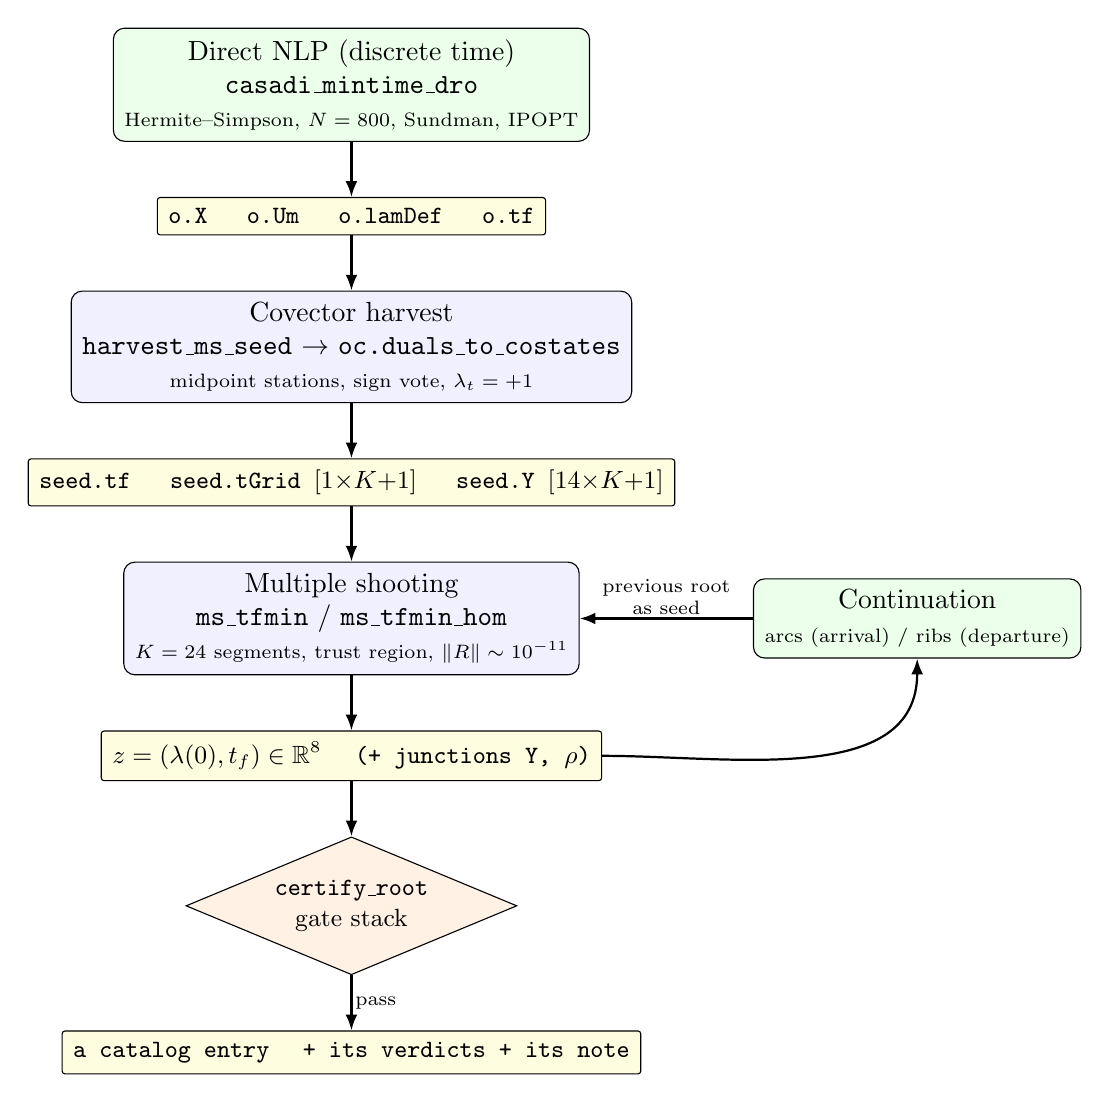
\begin{tikzpicture}[node distance=7mm]
\node[ext] (d) {Direct NLP (discrete time)\\\file{casadi\_mintime\_dro}\\{\scriptsize Hermite--Simpson, $N=800$, Sundman, IPOPT}};
\node[data,below=of d] (o) {o.X \quad o.Um \quad o.lamDef \quad o.tf};
\node[proc,below=of o] (h) {Covector harvest\\\file{harvest\_ms\_seed} $\to$ \file{oc.duals\_to\_costates}\\{\scriptsize midpoint stations, sign vote, $\lambda_t=+1$}};
\node[data,below=of h] (s) {seed.tf \quad seed.tGrid $[1{\times}K{+}1]$ \quad seed.Y $[14{\times}K{+}1]$};
\node[proc,below=of s] (m) {Multiple shooting\\\file{ms\_tfmin} / \file{ms\_tfmin\_hom}\\{\scriptsize $K=24$ segments, trust region, $\|R\|\sim10^{-11}$}};
\node[data,below=of m] (z) {$z=(\lambda(0),\tf)\in\R^8$ \; (+ junctions Y, $\rho$)};
\node[gate,below=of z,inner sep=3pt] (g) {\file{certify\_root}\\gate stack};
\node[data,below=of g] (e) {a catalog entry \; + its verdicts + its note};
\node[ext,right=22mm of m] (c) {Continuation\\{\scriptsize arcs (arrival) / ribs (departure)}};
\draw[arr] (d)--(o); \draw[arr] (o)--(h); \draw[arr] (h)--(s); \draw[arr] (s)--(m);
\draw[arr] (m)--(z); \draw[arr] (z)--(g); \draw[arr] (g)--node[lbl,right]{pass}(e);
\draw[arr] (c) -- node[lbl,above,align=center]{previous root\\as seed} (m);
\draw[arr] (z.east) to[out=0,in=-90] (c.south);
\end{tikzpicture}
\caption{The two ways into the shooting solve. The direct branch (left) pays
for a seed when no neighbour exists; the continuation branch (right) reuses
the previous converged root and is what produced most of the library.}
\end{figure}

\subsection{The gate stack: where a number becomes an entry}\label{sec:gates}

\begin{intu}
A converged root is not yet an answer. Newton's method converges to
\emph{stationary points}, and a stationary point of a shooting residual can
be a maximum, a saddle, a solution of a different problem, or a numerical
artefact. The gate stack is the campaign's answer to ``how do you know?'',
and it is deliberately redundant: the flight is re-integrated from $z$ alone
at tight tolerance, so a root that only looks converged in the solver's own
arithmetic is caught.
\end{intu}

\begin{rig}
\file{certify\_root} applies, in order, and stops at the first failure with a
named reason:
\begin{enumerate}[nosep]
\item multiple-shooting residual below \file{tolR} (a polish that plateaus is
      allowed through but \emph{says so} in the entry's reason and note);
\item the flown arrival: re-integrate from $z$ with ode113 at $10^{-13}$ and
      require the miss in \emph{position and velocity} below gates;
\item transversality $\lm(\tf)=0$ read off that tight flight (reading it off a
      loose flight cost the campaign five certified phases --- FINDINGS §59);
\item pointwise PMP checks along the arc: $\max|H|$, adjoint-equation
      residual, the minimum-principle gap (is the applied control actually
      the minimiser?), throttle $=1$;
\item a \file{pumpkyn tfMin} witness --- an independent solver reaching the
      same root;
\item the free-time conjugate test: the quotiented Jacobi determinant on a
      dense scan, no interior sign change (this is the Bonnard--Caillau--Trélat
      second-order test, and it refuted 12 of 14 candidates that passed every
      first-order check --- FINDINGS §38);
\item the BCT sufficiency hypotheses: strong Legendre $\min_t\|\lv\|>0$,
      $Q_{mt}>0$, and normality via $\dim S = 1$ with a $10\times$ margin;
\item lunar clearance $\ge 1900$\,km along the whole flight.
\end{enumerate}
\end{rig}

\subsection{The homogeneous chart}\label{sec:hom}

\begin{intu}
The costates of a min-time problem are defined only up to positive scaling in
the \emph{abnormal} case, and near a loss of normality the ordinary
normalisation ($\lambda_t=1$, say) becomes singular --- the solver's
unknowns run off to infinity while the trajectory stays perfectly finite.
Carrying an extra scalar $\rho$ and normalising $(\lambda,\rho)$ onto a
sphere removes the singularity: the walk passes smoothly through the place
where the ordinary chart would have died, and $\rho\to0$ becomes a
\emph{diagnosis} (``this family is losing normality here'') rather than a
crash.
\end{intu}

\begin{rig}
\file{ms\_tfmin\_hom} solves the same boundary-value problem with the
homogeneous unknown $(\lambda,\rho)$ normalised, and \file{ms\_bvp} carries
\file{nExtra} such scalars generically. In the arcs, $\rho$ is recorded at
every step; its minimum over a family and the phase where it occurs are part
of the family map, and \file{certify\_root} uses the normal chart for the
final polish so the shipped $z$ is in \file{tfMin}'s convention.
\end{rig}

%=========================================================================
\section{Economics: which route each entry took}
%=========================================================================

\begin{eli}
Solving from scratch is expensive; nudging a known answer is cheap. So we
solve from scratch only when we must --- to start a new family, or to fill a
cell nothing else can reach --- and nudge everywhere else.
\end{eli}

\begin{rig}
Of the 576 certified entries of the 70\,mN $24\times24$ library:
\begin{center}
\begin{tabular}{@{}lrl@{}}
\toprule
route & entries & seed \\
\midrule
rib continuation (departure axis) & 503 & the previous accepted rib point's junctions \\
arc crossing / registered root (spine) & 24 & the previous root on the arc, or a stored root \\
direct cell solve & 49 & a certified neighbour's PMP flight \\
\bottomrule
\end{tabular}
\end{center}
Costs: a rib point takes 2--10 minutes; an arc of 4000 steps takes 2--6
hours and yields tens of crossings; a direct cell solve takes 1--5 minutes
when it converges and burns its whole cap (300--900\,s) when it does not.
\end{rig}

\begin{meas}
\textbf{Seed geometry decides everything.} In the hole-filling pass, seeding
a direct solve from the neighbouring \emph{column} (a root at a different
arrival phase, however fast) sent IPOPT to 100--400-day junk, while seeding
from the same column's neighbour (same arrival geometry, adjacent departure
phase) converged in 1--3 minutes. The filler now tries same-column
neighbours first and caps the solve at 300\,s.

\textbf{And it decides across problems too.} Asked for the first root of a
\emph{different} problem --- DRO period $1\to2$ \emph{and} 7 $\to$ 8 petals
--- a direct solve warm-started from the 7-petal 70\,mN root returned a
259-day trajectory passing through the centre of the Moon. Changing only the
petal count ($\tau=1$, 7 $\to$ 8) still failed: 103 days, again through the
Moon. The arrival orbit's geometry, not the period, is what the warm start
cannot bridge. A new orbit pair therefore needs its own anchor route --- a
thrust ladder from a shipped catalog entry at the same orbit pair, or a
structured cold guess --- not a warm start from a different pair.
\end{meas}

\begin{warn}
A direct solve is \emph{branch-blind}: it lands in whatever basin its seed is
near, which is a feature when you are hunting for an unknown family and a
hazard when you assume it returns the family you started from. Four of the
library's five families were found precisely by exploiting this --- solving
at a phase where the known family was slow, warm-started from that known
family, and discovering the solver had landed somewhere else entirely, 5--7
days faster. Continuation would never have found them: it follows its own
sheet, faithfully, forever.
\end{warn}

%=========================================================================
\section{A worked reading of the code}
%=========================================================================

\begin{rig}
The shortest complete path through the library, for one transfer at
$(\sD,\sA)$:
\begin{enumerate}[nosep]
\item \file{arclength\_arrival('setup', so)} builds the physics closures $B$
      for the operating point: the two orbits' state functions
      $\bm x_D(\sD)$, $\bm x_A(\sA)$, the nondimensional thrust and exhaust
      speed, the residual and its parameter derivative. With
      \file{.physicsOnly} it stops there --- for a problem that has no root
      yet.
\item A seed by one of \S\ref{sec:three}'s three routes.
\item \file{ms\_tfmin(rv0, rvf, seed, Tmax, c, mu, opts)} $\to$ $z$,
      \file{info.Y} (junctions), \file{info.normR}; or
      \file{ms\_tfmin\_hom} for the homogeneous chart.
\item \file{certify\_root(seed, rv0, rvf, B, copts)} $\to$ a verdict struct:
      \file{.ok}, \file{.reason}, \file{.note}, $z$, $Y$, $\tf$ in days, the
      flown misses, the conjugate verdict, the three gate margins, the lift
      margin, wall time.
\item Packaging (\file{sheet\_to\_catalog\_file} $\to$
      \file{build\_costate\_catalog\_family}) carries only certified entries,
      with their verdicts, their family label and their provenance note.
\end{enumerate}
For a single transfer the front door \file{run\_dro\_tulip(sD, sA)} does all
of this and reports the route it took; for a whole library,
\file{run\_phase\_torus(spec)}.
\end{rig}

%=========================================================================
\section{Summary}
%=========================================================================

\begin{eli}
A seed is a rough draft of the entire trip --- positions and steering numbers
at 25 moments. You get one either by solving a cruder version of the problem
with a big optimiser (which hands you the steering numbers as a by-product),
or by nudging an answer you already have. Then a careful solver makes the
draft exact, and a stack of independent checks decides whether the result is
really the fastest trip and not just an arithmetic coincidence.
\end{eli}

\noindent
\begin{tabular}{@{}p{0.28\textwidth}p{0.68\textwidth}@{}}
\toprule
a seed is & a $14\times(K{+}1)$ state--costate trajectory plus $\tf$ and the junction times \\
it is not & a guess at $\lambda(0)$; single shooting from one misses by $10^4$--$10^5$\,km \\
made from & a direct solve's duals; an existing root's flight; the previous root of a continuation \\
consumed by & \file{ms\_tfmin} / \file{ms\_tfmin\_hom}, which return $z=(\lambda(0),\tf)$ \\
validated by & \file{certify\_root}: eight independent gates, each with a named failure \\
economics & 503 of 576 library entries came from continuation, 49 from direct cell solves, 24 from arcs and stored roots \\
\bottomrule
\end{tabular}

\end{document}
